%%%%%%%%%%%%%%%%%%%%%%%%%%%%%%%%%%%%%%%
% Wenneker Resume/CV
% LaTeX Template
% Version 1.1 (19/6/2016)
%
% This template has been downloaded from:
% http://www.LaTeXTemplates.com
%
% Original author:
% Frits Wenneker (http://www.howtotex.com) with extensive modifications by 
% Vel (vel@LaTeXTemplates.com)
%
% License:
% CC BY-NC-SA 3.0 (http://creativecommons.org/licenses/by-nc-sa/3.0/
%
%%%%%%%%%%%%%%%%%%%%%%%%%%%%%%%%%%%%%%

%----------------------------------------------------------------------------------------
% PACKAGES AND OTHER DOCUMENT CONFIGURATIONS
%----------------------------------------------------------------------------------------

\documentclass[a4paper,12pt]{memoir} % Font and paper size

\input{structure.tex} % Include the file specifying document layout and packages

%----------------------------------------------------------------------------------------
% NAME AND CONTACT INFORMATION 
%----------------------------------------------------------------------------------------

\userinformation{ % Set the content that goes into the sidebar of each page
\begin{flushright}
% Comment out this figure block if you don't want a photo
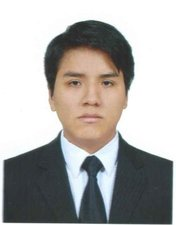
\includegraphics[width=0.6\columnwidth]{profile.jpg}\\[\baselineskip] % Your photo
\small % Smaller font size
Javier Huaman Adama \\ % Your name
\url{javier.adama@gmail} \\ % Your email address
(+51) 950450833 \\ % Your phone number
\Sep % Some whitespace
\textbf{Dirección} \\
Calle 3 de Mayo \\ % Address 1
Mz. A Lt. 8 Urb. El Bosque \\ % Address 2
Ate - Lima \\ % Address 3
\vfill % Whitespace under this block to push it up under the photo
\end{flushright}
}

%----------------------------------------------------------------------------------------

\begin{document}

\userinformation % Print your information in the left column

\framebreak % End of the first column

%----------------------------------------------------------------------------------------
% HEADING
%----------------------------------------------------------------------------------------

\cvheading{Javier Huaman Adama} % Large heading - your name

\cvsubheading{Téc. Computación e Infórmatica} % Subheading - your occupation/specialization

%----------------------------------------------------------------------------------------
% ABOUT ME
%----------------------------------------------------------------------------------------

\aboutme{Acerca de mi}{Soy proactivo, responsable, puntual y flexible a los cambios también me desenvuelvo mejor trabajando en grupo, me gusta formar parte de un ambiente laboral saludable. Me interesa trabajar en todo lo orientado al desarrollo de software (programación, prueba, despliegue e implementación).}

%----------------------------------------------------------------------------------------
% EDUCATION
%----------------------------------------------------------------------------------------

\CVSection{Educación}

%------------------------------------------------

\CVItem{2013 - 2015, CIBERTEC}{Técnico de Computación e Infórmatica}

%------------------------------------------------

\CVItem{2007 - 2012, Niño Jesús de Praga}{Secundaria completo.}

%------------------------------------------------

\Sep % Extra whitespace after the end of a major section

%----------------------------------------------------------------------------------------
% EXPERIENCE
%----------------------------------------------------------------------------------------

\CVSection{Experiencia}

%------------------------------------------------

\CVItem{Febrero 2015 - Marzo 2017, \textit{Desarrollador Web}, CAVASOFT SAC}{
\begin{itemize}
  \item Implementación de una solución tecnologica para el control de lavado de activos para Agentes de Aduana.
  Tecnologia usadas:
  \begin{itemize}
    \item Spring MVC, Spring Security, iText, MongoDB, Git, Maven, Tomcat.
  \end{itemize}
  \item Desarrollo de un software de asesor de comercio exterior para Agentes de Aduana.
  Tecnologia usadas:
  \begin{itemize}
    \item Spring MVC, Spring Security, SQL Server 2012, Bazaar, Maven, Tomcat.
  \end{itemize}
  \item Diseño de webservices para la generación de informe anual de registro de operaciones.
  Tecnologia usadas:
  \begin{itemize}
    \item Python(módulos especializados).
  \end{itemize}
\end{itemize}
}

\Sep % Extra whitespace after the end of a major section

%----------------------------------------------------------------------------------------
% SKILLS
%----------------------------------------------------------------------------------------

\CVSection{Conocimiento de Informática}

\CVItem{Lenguajes}
{\begin{tabular}{p{0.2\textwidth} p{0.2\textwidth} p{0.2\textwidth}}
\bluebullet Java &  \bluebullet Python & \bluebullet NodeJS\\
\bluebullet Unix Shell&  \bluebullet Ruby\\
\end{tabular}}

\CVItem{General}{
\begin{itemize}
  \item Frameworks
  \begin{itemize}
    \item J2EE (JSP, JSTL, Servlet),
          JSF (Primefaces),
          Spring (MVC, Spring security),
          Maven, JUnit, Struts2, GAE (Google AppEngine),
          Flask, Django, Express.
  \end{itemize}
  \item Base de Datos
  \begin{itemize}
    \item MySQL (Intermedio), SQL Server 2012 (Intermedio), Oracle (Básico), JPA, Hibernate, JDBC.
  \end{itemize}
  \item Sistema Operativos
  \begin{itemize}
    \item Windows (7, 8), Linux (Debian, Ubuntu, CentOS, openSUSE).
  \end{itemize}
  \item Web
  \begin{itemize}
    \item HTML, CSS, Jquery, JSON, XML, Frameworks visuales (SemanticUI, Bootstrap), JS.
  \end{itemize}
  \item Repositorios
  \begin{itemize}
    \item Git, Bazaar, Subversion.
  \end{itemize}
  \item Herramientas
  \begin{itemize}
    \item Sublime Text, Eclipse (Mars, Luna), MySQL Worbench.
  \end{itemize}
\end{itemize}
}

%------------------------------------------------

\Sep % Extra whitespace after the end of a major section

%----------------------------------------------------------------------------------------
% NEW PAGE DELIMITER
% Place this block wherever you would like the content of your CV to go onto the next page
%----------------------------------------------------------------------------------------

\clearpage % Start a new page

\userinformation % Print your information in the left column

\framebreak % End of the first column

%----------------------------------------------------------------------------------------
% COMMUNICATION SKILLS
%----------------------------------------------------------------------------------------

\CVSection{Proyectos Personales/Educativos}

%------------------------------------------------

\CVItem{Sistema de Control de Correo Electronico}{
Software para la administración de diversas cuentas de correo electronico
\begin{itemize}
  \item Tecnologia usadas:
  \begin{itemize}
    \item Java (Servlet, JSP, JSTL), MySQL, Maven, Git.
  \end{itemize}
\end{itemize}
}

%------------------------------------------------

\CVItem{Sistema de Reserva para un Cine}{
Se implemento un sistema con lenguaje Java que se alimenta de un web services
para los procesos de buscar cartelera, registrar una nueva reserva y buscar reserva.
\begin{itemize}
  \item Tecnologia usadas:
  \begin{itemize}
    \item Java Web Service, Java (Servlet, JSP, JSTL), Tomcat, MySQL, Maven, Git.
  \end{itemize}
\end{itemize}
}

%------------------------------------------------

\CVItem{Sistema de control de máquina remoto}{
Se implementó un sistema para el control de máquinas desde un servidor de manera remota.
(Envío de archivos, apagar/encender/reiniciar máquina). Mediante sockets usando Java.
\begin{itemize}
  \item Tecnologia usadas:
  \begin{itemize}
    \item Java sockets, Swing, Git.
  \end{itemize}
\end{itemize}
}

%------------------------------------------------

\CVItem{Sistema de Red Social}{
Se implementó un sistema en base de una red social.
\begin{itemize}
  \item Tecnologia usadas:
  \begin{itemize}
    \item Primefaces, JSF, MySql, JPA, Maven, JUnit, Git.
  \end{itemize}
\end{itemize}
}

%------------------------------------------------

\CVItem{Examen en linea}{
Se implementó un sistema permite realizar examenes en linea.
\begin{itemize}
  \item Tecnologia usadas:
  \begin{itemize}
    \item Primefaces, JSF, MySql, JPA, Maven, JUnit, Git.
  \end{itemize}
\end{itemize}
}

%------------------------------------------------

\Sep % Extra whitespace after the end of a major section


%----------------------------------------------------------------------------------------
% AWARDS
%----------------------------------------------------------------------------------------

\CVSection{Cursos y Seminarios}

%------------------------------------------------

\CVItem{2016, \textit{Diplomado en Innovación e Integración Tecnológia}, CIBERTEC}

%------------------------------------------------

\CVItem{2014, \textit{Intercambio AIEP-Conferencias}, AIEP-Chile}

%----------------------------------------------------------------------------------------
% Referencias
%----------------------------------------------------------------------------------------

\CVSection{Referencias}

%------------------------------------------------

\CVItem{Profesional}{
\begin{itemize}
  \item Github (\url{https://github.com/Hetaki})
  \item Launchpad (\url{https://launchpad.net/~jahanjp09})
  \item BitBucket (\url{https://bitbucket.org/JavierHuaman/})
  \item Udemy (\url{https://www.udemy.com/user/javier-antonio-huaman-adama/})
\end{itemize}
}

%------------------------------------------------

\CVItem{Social}{
\begin{itemize}
  \item Linkedin (\url{https://www.linkedin.com/in/javierhuaman})
\end{itemize}
}

%----------------------------------------------------------------------------------------

\end{document}
